% SOURCE: quant_survival_repair_v1.json fields cells.*.arms.*.{flat_rank,conditional_survival_given_fp32_worked,absolute_quantized_esr}.
% !TEX encoding = UTF-8 Unicode
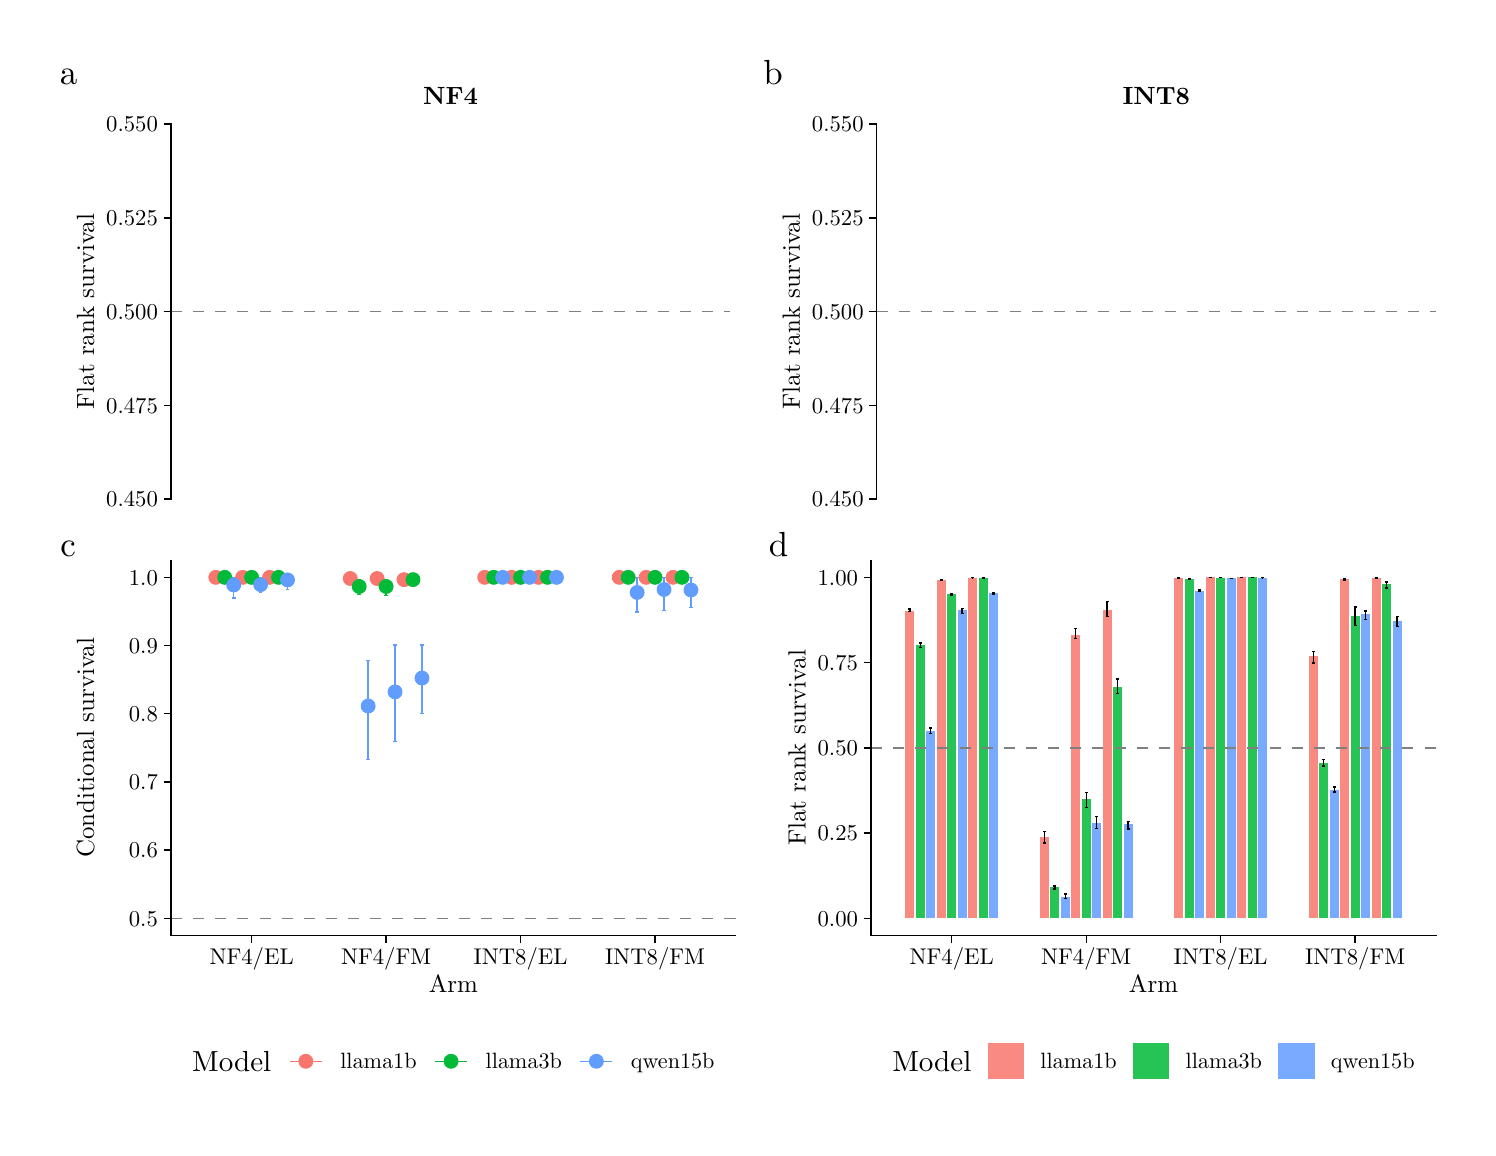
\begin{tikzpicture}[x=1pt,y=1pt]
\definecolor{fillColor}{RGB}{255,255,255}
\path[use as bounding box,fill=fillColor,fill opacity=0.00] (0,0) rectangle (520.34,397.48);
\begin{scope}
\path[clip] (  0.00,  0.00) rectangle (520.34,397.48);
\definecolor{drawColor}{RGB}{255,255,255}
\definecolor{fillColor}{RGB}{255,255,255}

\path[draw=drawColor,line width= 0.6pt,line join=round,line cap=round,fill=fillColor] (  0.00,  0.00) rectangle (520.34,397.48);
\end{scope}
\begin{scope}
\path[clip] (  5.50,221.13) rectangle (259.82,391.98);
\definecolor{drawColor}{RGB}{255,255,255}
\definecolor{fillColor}{RGB}{255,255,255}

\path[draw=drawColor,line width= 0.5pt,line join=round,line cap=round,fill=fillColor] (  5.50,221.13) rectangle (259.82,391.98);
\end{scope}
\begin{scope}
\path[clip] (259.82,221.13) rectangle (514.84,391.98);
\definecolor{drawColor}{RGB}{255,255,255}
\definecolor{fillColor}{RGB}{255,255,255}

\path[draw=drawColor,line width= 0.5pt,line join=round,line cap=round,fill=fillColor] (259.82,221.13) rectangle (514.84,391.98);
\end{scope}
\begin{scope}
\path[clip] ( 51.77,227.13) rectangle (253.82,362.65);
\definecolor{fillColor}{RGB}{255,255,255}

\path[fill=fillColor] ( 51.77,227.13) rectangle (253.82,362.65);
\definecolor{drawColor}{gray}{0.50}

\path[draw=drawColor,line width= 0.5pt,dash pattern=on 4pt off 4pt ,line join=round] ( 51.77,294.89) -- (253.82,294.89);
\end{scope}
\begin{scope}
\path[clip] (  0.00,  0.00) rectangle (520.34,397.48);
\definecolor{drawColor}{RGB}{0,0,0}

\path[draw=drawColor,line width= 0.5pt,line join=round,line cap=rect] ( 51.77,227.13) --
	( 51.77,362.65);
\end{scope}
\begin{scope}
\path[clip] (  0.00,  0.00) rectangle (520.34,397.48);
\definecolor{drawColor}{RGB}{0,0,0}

\node[text=drawColor,anchor=base east,inner sep=0pt, outer sep=0pt, scale=  0.82] at ( 47.04,224.31) {0.450};

\node[text=drawColor,anchor=base east,inner sep=0pt, outer sep=0pt, scale=  0.82] at ( 47.04,258.19) {0.475};

\node[text=drawColor,anchor=base east,inner sep=0pt, outer sep=0pt, scale=  0.82] at ( 47.04,292.07) {0.500};

\node[text=drawColor,anchor=base east,inner sep=0pt, outer sep=0pt, scale=  0.82] at ( 47.04,325.95) {0.525};

\node[text=drawColor,anchor=base east,inner sep=0pt, outer sep=0pt, scale=  0.82] at ( 47.04,359.82) {0.550};
\end{scope}
\begin{scope}
\path[clip] (  0.00,  0.00) rectangle (520.34,397.48);
\definecolor{drawColor}{RGB}{0,0,0}

\path[draw=drawColor,line width= 0.5pt,line join=round] ( 49.14,227.13) --
	( 51.77,227.13);

\path[draw=drawColor,line width= 0.5pt,line join=round] ( 49.14,261.01) --
	( 51.77,261.01);

\path[draw=drawColor,line width= 0.5pt,line join=round] ( 49.14,294.89) --
	( 51.77,294.89);

\path[draw=drawColor,line width= 0.5pt,line join=round] ( 49.14,328.77) --
	( 51.77,328.77);

\path[draw=drawColor,line width= 0.5pt,line join=round] ( 49.14,362.65) --
	( 51.77,362.65);
\end{scope}
\begin{scope}
\path[clip] (  0.00,  0.00) rectangle (520.34,397.48);
\definecolor{drawColor}{RGB}{0,0,0}

\node[text=drawColor,rotate= 90.00,anchor=base,inner sep=0pt, outer sep=0pt, scale=  0.90] at ( 24.00,294.89) {Flat rank survival};
\end{scope}
\begin{scope}
\path[clip] (  0.00,  0.00) rectangle (520.34,397.48);
\definecolor{drawColor}{RGB}{0,0,0}

\node[text=drawColor,anchor=base,inner sep=0pt, outer sep=0pt, scale=  0.90] at (152.80,369.65) {\bfseries NF4};
\end{scope}
\begin{scope}
\path[clip] (  0.00,  0.00) rectangle (520.34,397.48);
\definecolor{drawColor}{RGB}{0,0,0}

\node[text=drawColor,anchor=base,inner sep=0pt, outer sep=0pt, scale=  1.26] at ( 14.65,377.08) {a};
\end{scope}
\begin{scope}
\path[clip] (306.79,227.13) rectangle (508.84,362.65);
\definecolor{fillColor}{RGB}{255,255,255}

\path[fill=fillColor] (306.79,227.13) rectangle (508.84,362.65);
\definecolor{drawColor}{gray}{0.50}

\path[draw=drawColor,line width= 0.5pt,dash pattern=on 4pt off 4pt ,line join=round] (306.79,294.89) -- (508.84,294.89);
\end{scope}
\begin{scope}
\path[clip] (  0.00,  0.00) rectangle (520.34,397.48);
\definecolor{drawColor}{RGB}{0,0,0}

\path[draw=drawColor,line width= 0.5pt,line join=round,line cap=rect] (306.79,227.13) --
	(306.79,362.65);
\end{scope}
\begin{scope}
\path[clip] (  0.00,  0.00) rectangle (520.34,397.48);
\definecolor{drawColor}{RGB}{0,0,0}

\node[text=drawColor,anchor=base east,inner sep=0pt, outer sep=0pt, scale=  0.82] at (302.07,224.31) {0.450};

\node[text=drawColor,anchor=base east,inner sep=0pt, outer sep=0pt, scale=  0.82] at (302.07,258.19) {0.475};

\node[text=drawColor,anchor=base east,inner sep=0pt, outer sep=0pt, scale=  0.82] at (302.07,292.07) {0.500};

\node[text=drawColor,anchor=base east,inner sep=0pt, outer sep=0pt, scale=  0.82] at (302.07,325.95) {0.525};

\node[text=drawColor,anchor=base east,inner sep=0pt, outer sep=0pt, scale=  0.82] at (302.07,359.82) {0.550};
\end{scope}
\begin{scope}
\path[clip] (  0.00,  0.00) rectangle (520.34,397.48);
\definecolor{drawColor}{RGB}{0,0,0}

\path[draw=drawColor,line width= 0.5pt,line join=round] (304.17,227.13) --
	(306.79,227.13);

\path[draw=drawColor,line width= 0.5pt,line join=round] (304.17,261.01) --
	(306.79,261.01);

\path[draw=drawColor,line width= 0.5pt,line join=round] (304.17,294.89) --
	(306.79,294.89);

\path[draw=drawColor,line width= 0.5pt,line join=round] (304.17,328.77) --
	(306.79,328.77);

\path[draw=drawColor,line width= 0.5pt,line join=round] (304.17,362.65) --
	(306.79,362.65);
\end{scope}
\begin{scope}
\path[clip] (  0.00,  0.00) rectangle (520.34,397.48);
\definecolor{drawColor}{RGB}{0,0,0}

\node[text=drawColor,rotate= 90.00,anchor=base,inner sep=0pt, outer sep=0pt, scale=  0.90] at (279.02,294.89) {Flat rank survival};
\end{scope}
\begin{scope}
\path[clip] (  0.00,  0.00) rectangle (520.34,397.48);
\definecolor{drawColor}{RGB}{0,0,0}

\node[text=drawColor,anchor=base,inner sep=0pt, outer sep=0pt, scale=  0.90] at (407.82,369.65) {\bfseries INT8};
\end{scope}
\begin{scope}
\path[clip] (  0.00,  0.00) rectangle (520.34,397.48);
\definecolor{drawColor}{RGB}{0,0,0}

\node[text=drawColor,anchor=base,inner sep=0pt, outer sep=0pt, scale=  1.26] at (269.32,377.08) {b};
\end{scope}
\begin{scope}
\path[clip] (  5.50,  5.50) rectangle (261.87,221.13);
\definecolor{drawColor}{RGB}{255,255,255}
\definecolor{fillColor}{RGB}{255,255,255}

\path[draw=drawColor,line width= 0.5pt,line join=round,line cap=round,fill=fillColor] (  5.50,  5.50) rectangle (261.87,221.13);
\end{scope}
\begin{scope}
\path[clip] (261.87,  5.50) rectangle (514.84,221.13);
\definecolor{drawColor}{RGB}{255,255,255}
\definecolor{fillColor}{RGB}{255,255,255}

\path[draw=drawColor,line width= 0.5pt,line join=round,line cap=round,fill=fillColor] (261.87,  5.50) rectangle (514.84,221.13);
\end{scope}
\begin{scope}
\path[clip] ( 51.77, 69.49) rectangle (255.87,205.01);
\definecolor{fillColor}{RGB}{255,255,255}

\path[fill=fillColor] ( 51.77, 69.49) rectangle (255.87,205.01);
\definecolor{drawColor}{RGB}{248,118,109}

\path[draw=drawColor,line width= 0.5pt,line join=round] ( 67.29,198.85) --
	( 68.64,198.85);

\path[draw=drawColor,line width= 0.5pt,line join=round] ( 67.97,198.85) --
	( 67.97,198.85);

\path[draw=drawColor,line width= 0.5pt,line join=round] ( 67.29,198.85) --
	( 68.64,198.85);

\path[draw=drawColor,line width= 0.5pt,line join=round] (115.89,198.85) --
	(117.24,198.85);

\path[draw=drawColor,line width= 0.5pt,line join=round] (116.56,198.85) --
	(116.56,197.19);

\path[draw=drawColor,line width= 0.5pt,line join=round] (115.89,197.19) --
	(117.24,197.19);

\path[draw=drawColor,line width= 0.5pt,line join=round] (164.48,198.85) --
	(165.83,198.85);

\path[draw=drawColor,line width= 0.5pt,line join=round] (165.16,198.85) --
	(165.16,198.85);

\path[draw=drawColor,line width= 0.5pt,line join=round] (164.48,198.85) --
	(165.83,198.85);

\path[draw=drawColor,line width= 0.5pt,line join=round] (213.08,198.85) --
	(214.43,198.85);

\path[draw=drawColor,line width= 0.5pt,line join=round] (213.76,198.85) --
	(213.76,198.85);

\path[draw=drawColor,line width= 0.5pt,line join=round] (213.08,198.85) --
	(214.43,198.85);

\path[draw=drawColor,line width= 0.5pt,line join=round] ( 77.01,198.85) --
	( 78.36,198.85);

\path[draw=drawColor,line width= 0.5pt,line join=round] ( 77.69,198.85) --
	( 77.69,198.85);

\path[draw=drawColor,line width= 0.5pt,line join=round] ( 77.01,198.85) --
	( 78.36,198.85);

\path[draw=drawColor,line width= 0.5pt,line join=round] (125.61,198.85) --
	(126.96,198.85);

\path[draw=drawColor,line width= 0.5pt,line join=round] (126.28,198.85) --
	(126.28,196.98);

\path[draw=drawColor,line width= 0.5pt,line join=round] (125.61,196.98) --
	(126.96,196.98);

\path[draw=drawColor,line width= 0.5pt,line join=round] (174.20,198.85) --
	(175.55,198.85);

\path[draw=drawColor,line width= 0.5pt,line join=round] (174.88,198.85) --
	(174.88,198.85);

\path[draw=drawColor,line width= 0.5pt,line join=round] (174.20,198.85) --
	(175.55,198.85);

\path[draw=drawColor,line width= 0.5pt,line join=round] (222.80,198.85) --
	(224.15,198.85);

\path[draw=drawColor,line width= 0.5pt,line join=round] (223.47,198.85) --
	(223.47,198.85);

\path[draw=drawColor,line width= 0.5pt,line join=round] (222.80,198.85) --
	(224.15,198.85);

\path[draw=drawColor,line width= 0.5pt,line join=round] ( 86.73,198.85) --
	( 88.08,198.85);

\path[draw=drawColor,line width= 0.5pt,line join=round] ( 87.41,198.85) --
	( 87.41,198.85);

\path[draw=drawColor,line width= 0.5pt,line join=round] ( 86.73,198.85) --
	( 88.08,198.85);

\path[draw=drawColor,line width= 0.5pt,line join=round] (135.33,198.85) --
	(136.68,198.85);

\path[draw=drawColor,line width= 0.5pt,line join=round] (136.00,198.85) --
	(136.00,195.93);

\path[draw=drawColor,line width= 0.5pt,line join=round] (135.33,195.93) --
	(136.68,195.93);

\path[draw=drawColor,line width= 0.5pt,line join=round] (183.92,198.85) --
	(185.27,198.85);

\path[draw=drawColor,line width= 0.5pt,line join=round] (184.60,198.85) --
	(184.60,198.85);

\path[draw=drawColor,line width= 0.5pt,line join=round] (183.92,198.85) --
	(185.27,198.85);

\path[draw=drawColor,line width= 0.5pt,line join=round] (232.52,198.85) --
	(233.87,198.85);

\path[draw=drawColor,line width= 0.5pt,line join=round] (233.19,198.85) --
	(233.19,198.85);

\path[draw=drawColor,line width= 0.5pt,line join=round] (232.52,198.85) --
	(233.87,198.85);
\definecolor{drawColor}{RGB}{0,186,56}

\path[draw=drawColor,line width= 0.5pt,line join=round] ( 70.53,198.85) --
	( 71.88,198.85);

\path[draw=drawColor,line width= 0.5pt,line join=round] ( 71.21,198.85) --
	( 71.21,198.85);

\path[draw=drawColor,line width= 0.5pt,line join=round] ( 70.53,198.85) --
	( 71.88,198.85);

\path[draw=drawColor,line width= 0.5pt,line join=round] (119.13,198.02) --
	(120.48,198.02);

\path[draw=drawColor,line width= 0.5pt,line join=round] (119.80,198.02) --
	(119.80,192.67);

\path[draw=drawColor,line width= 0.5pt,line join=round] (119.13,192.67) --
	(120.48,192.67);

\path[draw=drawColor,line width= 0.5pt,line join=round] (167.72,198.85) --
	(169.07,198.85);

\path[draw=drawColor,line width= 0.5pt,line join=round] (168.40,198.85) --
	(168.40,198.85);

\path[draw=drawColor,line width= 0.5pt,line join=round] (167.72,198.85) --
	(169.07,198.85);

\path[draw=drawColor,line width= 0.5pt,line join=round] (216.32,198.85) --
	(217.67,198.85);

\path[draw=drawColor,line width= 0.5pt,line join=round] (217.00,198.85) --
	(217.00,198.85);

\path[draw=drawColor,line width= 0.5pt,line join=round] (216.32,198.85) --
	(217.67,198.85);

\path[draw=drawColor,line width= 0.5pt,line join=round] ( 80.25,198.85) --
	( 81.60,198.85);

\path[draw=drawColor,line width= 0.5pt,line join=round] ( 80.93,198.85) --
	( 80.93,198.85);

\path[draw=drawColor,line width= 0.5pt,line join=round] ( 80.25,198.85) --
	( 81.60,198.85);

\path[draw=drawColor,line width= 0.5pt,line join=round] (128.85,198.03) --
	(130.20,198.03);

\path[draw=drawColor,line width= 0.5pt,line join=round] (129.52,198.03) --
	(129.52,192.28);

\path[draw=drawColor,line width= 0.5pt,line join=round] (128.85,192.28) --
	(130.20,192.28);

\path[draw=drawColor,line width= 0.5pt,line join=round] (177.44,198.85) --
	(178.79,198.85);

\path[draw=drawColor,line width= 0.5pt,line join=round] (178.12,198.85) --
	(178.12,198.85);

\path[draw=drawColor,line width= 0.5pt,line join=round] (177.44,198.85) --
	(178.79,198.85);

\path[draw=drawColor,line width= 0.5pt,line join=round] (226.04,198.85) --
	(227.39,198.85);

\path[draw=drawColor,line width= 0.5pt,line join=round] (226.71,198.85) --
	(226.71,198.85);

\path[draw=drawColor,line width= 0.5pt,line join=round] (226.04,198.85) --
	(227.39,198.85);

\path[draw=drawColor,line width= 0.5pt,line join=round] ( 89.97,198.85) --
	( 91.32,198.85);

\path[draw=drawColor,line width= 0.5pt,line join=round] ( 90.65,198.85) --
	( 90.65,198.85);

\path[draw=drawColor,line width= 0.5pt,line join=round] ( 89.97,198.85) --
	( 91.32,198.85);

\path[draw=drawColor,line width= 0.5pt,line join=round] (138.57,198.85) --
	(139.92,198.85);

\path[draw=drawColor,line width= 0.5pt,line join=round] (139.24,198.85) --
	(139.24,196.38);

\path[draw=drawColor,line width= 0.5pt,line join=round] (138.57,196.38) --
	(139.92,196.38);

\path[draw=drawColor,line width= 0.5pt,line join=round] (187.16,198.85) --
	(188.51,198.85);

\path[draw=drawColor,line width= 0.5pt,line join=round] (187.84,198.85) --
	(187.84,198.85);

\path[draw=drawColor,line width= 0.5pt,line join=round] (187.16,198.85) --
	(188.51,198.85);

\path[draw=drawColor,line width= 0.5pt,line join=round] (235.76,198.85) --
	(237.11,198.85);

\path[draw=drawColor,line width= 0.5pt,line join=round] (236.43,198.85) --
	(236.43,198.85);

\path[draw=drawColor,line width= 0.5pt,line join=round] (235.76,198.85) --
	(237.11,198.85);
\definecolor{drawColor}{RGB}{97,156,255}

\path[draw=drawColor,line width= 0.5pt,line join=round] ( 73.77,198.85) --
	( 75.12,198.85);

\path[draw=drawColor,line width= 0.5pt,line join=round] ( 74.45,198.85) --
	( 74.45,191.42);

\path[draw=drawColor,line width= 0.5pt,line join=round] ( 73.77,191.42) --
	( 75.12,191.42);

\path[draw=drawColor,line width= 0.5pt,line join=round] (122.37,168.77) --
	(123.72,168.77);

\path[draw=drawColor,line width= 0.5pt,line join=round] (123.04,168.77) --
	(123.04,133.11);

\path[draw=drawColor,line width= 0.5pt,line join=round] (122.37,133.11) --
	(123.72,133.11);

\path[draw=drawColor,line width= 0.5pt,line join=round] (170.96,198.85) --
	(172.31,198.85);

\path[draw=drawColor,line width= 0.5pt,line join=round] (171.64,198.85) --
	(171.64,198.85);

\path[draw=drawColor,line width= 0.5pt,line join=round] (170.96,198.85) --
	(172.31,198.85);

\path[draw=drawColor,line width= 0.5pt,line join=round] (219.56,198.85) --
	(220.91,198.85);

\path[draw=drawColor,line width= 0.5pt,line join=round] (220.23,198.85) --
	(220.23,186.38);

\path[draw=drawColor,line width= 0.5pt,line join=round] (219.56,186.38) --
	(220.91,186.38);

\path[draw=drawColor,line width= 0.5pt,line join=round] ( 83.49,198.85) --
	( 84.84,198.85);

\path[draw=drawColor,line width= 0.5pt,line join=round] ( 84.17,198.85) --
	( 84.17,193.27);

\path[draw=drawColor,line width= 0.5pt,line join=round] ( 83.49,193.27) --
	( 84.84,193.27);

\path[draw=drawColor,line width= 0.5pt,line join=round] (132.09,174.42) --
	(133.44,174.42);

\path[draw=drawColor,line width= 0.5pt,line join=round] (132.76,174.42) --
	(132.76,139.57);

\path[draw=drawColor,line width= 0.5pt,line join=round] (132.09,139.57) --
	(133.44,139.57);

\path[draw=drawColor,line width= 0.5pt,line join=round] (180.68,198.85) --
	(182.03,198.85);

\path[draw=drawColor,line width= 0.5pt,line join=round] (181.36,198.85) --
	(181.36,198.85);

\path[draw=drawColor,line width= 0.5pt,line join=round] (180.68,198.85) --
	(182.03,198.85);

\path[draw=drawColor,line width= 0.5pt,line join=round] (229.28,198.85) --
	(230.63,198.85);

\path[draw=drawColor,line width= 0.5pt,line join=round] (229.95,198.85) --
	(229.95,186.97);

\path[draw=drawColor,line width= 0.5pt,line join=round] (229.28,186.97) --
	(230.63,186.97);

\path[draw=drawColor,line width= 0.5pt,line join=round] ( 93.21,198.85) --
	( 94.56,198.85);

\path[draw=drawColor,line width= 0.5pt,line join=round] ( 93.89,198.85) --
	( 93.89,194.50);

\path[draw=drawColor,line width= 0.5pt,line join=round] ( 93.21,194.50) --
	( 94.56,194.50);

\path[draw=drawColor,line width= 0.5pt,line join=round] (141.81,174.35) --
	(143.16,174.35);

\path[draw=drawColor,line width= 0.5pt,line join=round] (142.48,174.35) --
	(142.48,149.66);

\path[draw=drawColor,line width= 0.5pt,line join=round] (141.81,149.66) --
	(143.16,149.66);

\path[draw=drawColor,line width= 0.5pt,line join=round] (190.40,198.85) --
	(191.75,198.85);

\path[draw=drawColor,line width= 0.5pt,line join=round] (191.08,198.85) --
	(191.08,198.85);

\path[draw=drawColor,line width= 0.5pt,line join=round] (190.40,198.85) --
	(191.75,198.85);

\path[draw=drawColor,line width= 0.5pt,line join=round] (239.00,198.85) --
	(240.35,198.85);

\path[draw=drawColor,line width= 0.5pt,line join=round] (239.67,198.85) --
	(239.67,188.02);

\path[draw=drawColor,line width= 0.5pt,line join=round] (239.00,188.02) --
	(240.35,188.02);
\definecolor{drawColor}{RGB}{248,118,109}
\definecolor{fillColor}{RGB}{248,118,109}

\path[draw=drawColor,line width= 0.4pt,line join=round,line cap=round,fill=fillColor] ( 67.97,198.85) circle (  2.48);

\path[draw=drawColor,line width= 0.4pt,line join=round,line cap=round,fill=fillColor] (116.56,198.43) circle (  2.48);

\path[draw=drawColor,line width= 0.4pt,line join=round,line cap=round,fill=fillColor] (165.16,198.85) circle (  2.48);

\path[draw=drawColor,line width= 0.4pt,line join=round,line cap=round,fill=fillColor] (213.76,198.85) circle (  2.48);

\path[draw=drawColor,line width= 0.4pt,line join=round,line cap=round,fill=fillColor] ( 77.69,198.85) circle (  2.48);

\path[draw=drawColor,line width= 0.4pt,line join=round,line cap=round,fill=fillColor] (126.28,198.43) circle (  2.48);

\path[draw=drawColor,line width= 0.4pt,line join=round,line cap=round,fill=fillColor] (174.88,198.85) circle (  2.48);

\path[draw=drawColor,line width= 0.4pt,line join=round,line cap=round,fill=fillColor] (223.47,198.85) circle (  2.48);

\path[draw=drawColor,line width= 0.4pt,line join=round,line cap=round,fill=fillColor] ( 87.41,198.85) circle (  2.48);

\path[draw=drawColor,line width= 0.4pt,line join=round,line cap=round,fill=fillColor] (136.00,198.02) circle (  2.48);

\path[draw=drawColor,line width= 0.4pt,line join=round,line cap=round,fill=fillColor] (184.60,198.85) circle (  2.48);

\path[draw=drawColor,line width= 0.4pt,line join=round,line cap=round,fill=fillColor] (233.19,198.85) circle (  2.48);
\definecolor{drawColor}{RGB}{0,186,56}
\definecolor{fillColor}{RGB}{0,186,56}

\path[draw=drawColor,line width= 0.4pt,line join=round,line cap=round,fill=fillColor] ( 71.21,198.85) circle (  2.48);

\path[draw=drawColor,line width= 0.4pt,line join=round,line cap=round,fill=fillColor] (119.80,195.55) circle (  2.48);

\path[draw=drawColor,line width= 0.4pt,line join=round,line cap=round,fill=fillColor] (168.40,198.85) circle (  2.48);

\path[draw=drawColor,line width= 0.4pt,line join=round,line cap=round,fill=fillColor] (217.00,198.85) circle (  2.48);

\path[draw=drawColor,line width= 0.4pt,line join=round,line cap=round,fill=fillColor] ( 80.93,198.85) circle (  2.48);

\path[draw=drawColor,line width= 0.4pt,line join=round,line cap=round,fill=fillColor] (129.52,195.56) circle (  2.48);

\path[draw=drawColor,line width= 0.4pt,line join=round,line cap=round,fill=fillColor] (178.12,198.85) circle (  2.48);

\path[draw=drawColor,line width= 0.4pt,line join=round,line cap=round,fill=fillColor] (226.71,198.85) circle (  2.48);

\path[draw=drawColor,line width= 0.4pt,line join=round,line cap=round,fill=fillColor] ( 90.65,198.85) circle (  2.48);

\path[draw=drawColor,line width= 0.4pt,line join=round,line cap=round,fill=fillColor] (139.24,198.03) circle (  2.48);

\path[draw=drawColor,line width= 0.4pt,line join=round,line cap=round,fill=fillColor] (187.84,198.85) circle (  2.48);

\path[draw=drawColor,line width= 0.4pt,line join=round,line cap=round,fill=fillColor] (236.43,198.85) circle (  2.48);
\definecolor{drawColor}{RGB}{97,156,255}
\definecolor{fillColor}{RGB}{97,156,255}

\path[draw=drawColor,line width= 0.4pt,line join=round,line cap=round,fill=fillColor] ( 74.45,196.10) circle (  2.48);

\path[draw=drawColor,line width= 0.4pt,line join=round,line cap=round,fill=fillColor] (123.04,152.35) circle (  2.48);

\path[draw=drawColor,line width= 0.4pt,line join=round,line cap=round,fill=fillColor] (171.64,198.85) circle (  2.48);

\path[draw=drawColor,line width= 0.4pt,line join=round,line cap=round,fill=fillColor] (220.23,193.39) circle (  2.48);

\path[draw=drawColor,line width= 0.4pt,line join=round,line cap=round,fill=fillColor] ( 84.17,196.22) circle (  2.48);

\path[draw=drawColor,line width= 0.4pt,line join=round,line cap=round,fill=fillColor] (132.76,157.47) circle (  2.48);

\path[draw=drawColor,line width= 0.4pt,line join=round,line cap=round,fill=fillColor] (181.36,198.85) circle (  2.48);

\path[draw=drawColor,line width= 0.4pt,line join=round,line cap=round,fill=fillColor] (229.95,194.46) circle (  2.48);

\path[draw=drawColor,line width= 0.4pt,line join=round,line cap=round,fill=fillColor] ( 93.89,197.93) circle (  2.48);

\path[draw=drawColor,line width= 0.4pt,line join=round,line cap=round,fill=fillColor] (142.48,162.46) circle (  2.48);

\path[draw=drawColor,line width= 0.4pt,line join=round,line cap=round,fill=fillColor] (191.08,198.85) circle (  2.48);

\path[draw=drawColor,line width= 0.4pt,line join=round,line cap=round,fill=fillColor] (239.67,194.28) circle (  2.48);
\definecolor{drawColor}{gray}{0.50}

\path[draw=drawColor,line width= 0.5pt,dash pattern=on 4pt off 4pt ,line join=round] ( 51.77, 75.65) -- (255.87, 75.65);
\end{scope}
\begin{scope}
\path[clip] (  0.00,  0.00) rectangle (520.34,397.48);
\definecolor{drawColor}{RGB}{0,0,0}

\path[draw=drawColor,line width= 0.5pt,line join=round,line cap=rect] ( 51.77, 69.49) --
	( 51.77,205.01);
\end{scope}
\begin{scope}
\path[clip] (  0.00,  0.00) rectangle (520.34,397.48);
\definecolor{drawColor}{RGB}{0,0,0}

\node[text=drawColor,anchor=base east,inner sep=0pt, outer sep=0pt, scale=  0.82] at ( 47.04, 72.83) {0.5};

\node[text=drawColor,anchor=base east,inner sep=0pt, outer sep=0pt, scale=  0.82] at ( 47.04, 97.47) {0.6};

\node[text=drawColor,anchor=base east,inner sep=0pt, outer sep=0pt, scale=  0.82] at ( 47.04,122.11) {0.7};

\node[text=drawColor,anchor=base east,inner sep=0pt, outer sep=0pt, scale=  0.82] at ( 47.04,146.75) {0.8};

\node[text=drawColor,anchor=base east,inner sep=0pt, outer sep=0pt, scale=  0.82] at ( 47.04,171.38) {0.9};

\node[text=drawColor,anchor=base east,inner sep=0pt, outer sep=0pt, scale=  0.82] at ( 47.04,196.02) {1.0};
\end{scope}
\begin{scope}
\path[clip] (  0.00,  0.00) rectangle (520.34,397.48);
\definecolor{drawColor}{RGB}{0,0,0}

\path[draw=drawColor,line width= 0.5pt,line join=round] ( 49.14, 75.65) --
	( 51.77, 75.65);

\path[draw=drawColor,line width= 0.5pt,line join=round] ( 49.14,100.29) --
	( 51.77,100.29);

\path[draw=drawColor,line width= 0.5pt,line join=round] ( 49.14,124.93) --
	( 51.77,124.93);

\path[draw=drawColor,line width= 0.5pt,line join=round] ( 49.14,149.57) --
	( 51.77,149.57);

\path[draw=drawColor,line width= 0.5pt,line join=round] ( 49.14,174.21) --
	( 51.77,174.21);

\path[draw=drawColor,line width= 0.5pt,line join=round] ( 49.14,198.85) --
	( 51.77,198.85);
\end{scope}
\begin{scope}
\path[clip] (  0.00,  0.00) rectangle (520.34,397.48);
\definecolor{drawColor}{RGB}{0,0,0}

\path[draw=drawColor,line width= 0.5pt,line join=round,line cap=rect] ( 51.77, 69.49) --
	(255.87, 69.49);
\end{scope}
\begin{scope}
\path[clip] (  0.00,  0.00) rectangle (520.34,397.48);
\definecolor{drawColor}{RGB}{0,0,0}

\path[draw=drawColor,line width= 0.5pt,line join=round] ( 80.93, 66.87) --
	( 80.93, 69.49);

\path[draw=drawColor,line width= 0.5pt,line join=round] (129.52, 66.87) --
	(129.52, 69.49);

\path[draw=drawColor,line width= 0.5pt,line join=round] (178.12, 66.87) --
	(178.12, 69.49);

\path[draw=drawColor,line width= 0.5pt,line join=round] (226.71, 66.87) --
	(226.71, 69.49);
\end{scope}
\begin{scope}
\path[clip] (  0.00,  0.00) rectangle (520.34,397.48);
\definecolor{drawColor}{RGB}{0,0,0}

\node[text=drawColor,anchor=base,inner sep=0pt, outer sep=0pt, scale=  0.82] at ( 80.93, 59.12) {NF4/EL};

\node[text=drawColor,anchor=base,inner sep=0pt, outer sep=0pt, scale=  0.82] at (129.52, 59.12) {NF4/FM};

\node[text=drawColor,anchor=base,inner sep=0pt, outer sep=0pt, scale=  0.82] at (178.12, 59.12) {INT8/EL};

\node[text=drawColor,anchor=base,inner sep=0pt, outer sep=0pt, scale=  0.82] at (226.71, 59.12) {INT8/FM};
\end{scope}
\begin{scope}
\path[clip] (  0.00,  0.00) rectangle (520.34,397.48);
\definecolor{drawColor}{RGB}{0,0,0}

\node[text=drawColor,anchor=base,inner sep=0pt, outer sep=0pt, scale=  0.90] at (153.82, 48.70) {Arm};
\end{scope}
\begin{scope}
\path[clip] (  0.00,  0.00) rectangle (520.34,397.48);
\definecolor{drawColor}{RGB}{0,0,0}

\node[text=drawColor,rotate= 90.00,anchor=base,inner sep=0pt, outer sep=0pt, scale=  0.90] at ( 24.00,137.25) {Conditional survival};
\end{scope}
\begin{scope}
\path[clip] (  0.00,  0.00) rectangle (520.34,397.48);
\definecolor{fillColor}{RGB}{255,255,255}

\path[fill=fillColor] ( 54.20, 11.50) rectangle (253.45, 36.45);
\end{scope}
\begin{scope}
\path[clip] (  0.00,  0.00) rectangle (520.34,397.48);
\definecolor{drawColor}{RGB}{0,0,0}

\node[text=drawColor,anchor=base west,inner sep=0pt, outer sep=0pt, scale=  1.05] at ( 59.45, 20.36) {Model};
\end{scope}
\begin{scope}
\path[clip] (  0.00,  0.00) rectangle (520.34,397.48);
\definecolor{fillColor}{RGB}{255,255,255}

\path[fill=fillColor] ( 93.27, 16.75) rectangle (107.73, 31.20);
\definecolor{drawColor}{RGB}{248,118,109}

\path[draw=drawColor,line width= 0.5pt,line join=round] ( 94.72, 23.98) -- (106.28, 23.98);
\definecolor{fillColor}{RGB}{248,118,109}

\path[draw=drawColor,line width= 0.4pt,line join=round,line cap=round,fill=fillColor] (100.50, 23.98) circle (  2.48);
\end{scope}
\begin{scope}
\path[clip] (  0.00,  0.00) rectangle (520.34,397.48);
\definecolor{fillColor}{RGB}{255,255,255}

\path[fill=fillColor] (145.77, 16.75) rectangle (160.23, 31.20);
\definecolor{drawColor}{RGB}{0,186,56}

\path[draw=drawColor,line width= 0.5pt,line join=round] (147.22, 23.98) -- (158.78, 23.98);
\definecolor{fillColor}{RGB}{0,186,56}

\path[draw=drawColor,line width= 0.4pt,line join=round,line cap=round,fill=fillColor] (153.00, 23.98) circle (  2.48);
\end{scope}
\begin{scope}
\path[clip] (  0.00,  0.00) rectangle (520.34,397.48);
\definecolor{fillColor}{RGB}{255,255,255}

\path[fill=fillColor] (198.28, 16.75) rectangle (212.73, 31.20);
\definecolor{drawColor}{RGB}{97,156,255}

\path[draw=drawColor,line width= 0.5pt,line join=round] (199.72, 23.98) -- (211.29, 23.98);
\definecolor{fillColor}{RGB}{97,156,255}

\path[draw=drawColor,line width= 0.4pt,line join=round,line cap=round,fill=fillColor] (205.50, 23.98) circle (  2.48);
\end{scope}
\begin{scope}
\path[clip] (  0.00,  0.00) rectangle (520.34,397.48);
\definecolor{drawColor}{RGB}{0,0,0}

\node[text=drawColor,anchor=base west,inner sep=0pt, outer sep=0pt, scale=  0.80] at (112.98, 21.22) {llama1b};
\end{scope}
\begin{scope}
\path[clip] (  0.00,  0.00) rectangle (520.34,397.48);
\definecolor{drawColor}{RGB}{0,0,0}

\node[text=drawColor,anchor=base west,inner sep=0pt, outer sep=0pt, scale=  0.80] at (165.48, 21.22) {llama3b};
\end{scope}
\begin{scope}
\path[clip] (  0.00,  0.00) rectangle (520.34,397.48);
\definecolor{drawColor}{RGB}{0,0,0}

\node[text=drawColor,anchor=base west,inner sep=0pt, outer sep=0pt, scale=  0.80] at (217.98, 21.22) {qwen15b};
\end{scope}
\begin{scope}
\path[clip] (  0.00,  0.00) rectangle (520.34,397.48);
\definecolor{drawColor}{RGB}{0,0,0}

\node[text=drawColor,anchor=base,inner sep=0pt, outer sep=0pt, scale=  1.26] at ( 14.65,206.23) {c};
\end{scope}
\begin{scope}
\path[clip] (304.74, 69.49) rectangle (508.84,205.01);
\definecolor{fillColor}{RGB}{255,255,255}

\path[fill=fillColor] (304.74, 69.49) rectangle (508.84,205.01);
\definecolor{fillColor}{RGB}{248,118,109}

\path[fill=fillColor,fill opacity=0.85] (317.16, 75.65) rectangle (320.40,186.86);

\path[fill=fillColor,fill opacity=0.85] (365.76, 75.65) rectangle (369.00,104.97);

\path[fill=fillColor,fill opacity=0.85] (414.35, 75.65) rectangle (417.59,198.59);

\path[fill=fillColor,fill opacity=0.85] (462.95, 75.65) rectangle (466.19,170.37);

\path[fill=fillColor,fill opacity=0.85] (328.50, 75.65) rectangle (331.74,197.99);

\path[fill=fillColor,fill opacity=0.85] (377.10, 75.65) rectangle (380.34,178.14);

\path[fill=fillColor,fill opacity=0.85] (425.69, 75.65) rectangle (428.93,198.83);

\path[fill=fillColor,fill opacity=0.85] (474.29, 75.65) rectangle (477.53,198.19);

\path[fill=fillColor,fill opacity=0.85] (339.84, 75.65) rectangle (343.08,198.77);

\path[fill=fillColor,fill opacity=0.85] (388.43, 75.65) rectangle (391.67,187.00);

\path[fill=fillColor,fill opacity=0.85] (437.03, 75.65) rectangle (440.27,198.85);

\path[fill=fillColor,fill opacity=0.85] (485.63, 75.65) rectangle (488.87,198.56);
\definecolor{fillColor}{RGB}{0,186,56}

\path[fill=fillColor,fill opacity=0.85] (320.94, 75.65) rectangle (324.18,174.24);

\path[fill=fillColor,fill opacity=0.85] (369.54, 75.65) rectangle (372.78, 86.89);

\path[fill=fillColor,fill opacity=0.85] (418.13, 75.65) rectangle (421.37,198.22);

\path[fill=fillColor,fill opacity=0.85] (466.73, 75.65) rectangle (469.97,131.76);

\path[fill=fillColor,fill opacity=0.85] (332.28, 75.65) rectangle (335.52,192.71);

\path[fill=fillColor,fill opacity=0.85] (380.88, 75.65) rectangle (384.12,118.68);

\path[fill=fillColor,fill opacity=0.85] (429.47, 75.65) rectangle (432.71,198.77);

\path[fill=fillColor,fill opacity=0.85] (478.07, 75.65) rectangle (481.31,184.90);

\path[fill=fillColor,fill opacity=0.85] (343.62, 75.65) rectangle (346.86,198.66);

\path[fill=fillColor,fill opacity=0.85] (392.21, 75.65) rectangle (395.45,159.39);

\path[fill=fillColor,fill opacity=0.85] (440.81, 75.65) rectangle (444.05,198.85);

\path[fill=fillColor,fill opacity=0.85] (489.41, 75.65) rectangle (492.65,196.28);
\definecolor{fillColor}{RGB}{97,156,255}

\path[fill=fillColor,fill opacity=0.85] (324.72, 75.65) rectangle (327.96,143.49);

\path[fill=fillColor,fill opacity=0.85] (373.32, 75.65) rectangle (376.56, 83.37);

\path[fill=fillColor,fill opacity=0.85] (421.91, 75.65) rectangle (425.15,194.09);

\path[fill=fillColor,fill opacity=0.85] (470.51, 75.65) rectangle (473.75,122.09);

\path[fill=fillColor,fill opacity=0.85] (336.06, 75.65) rectangle (339.30,186.99);

\path[fill=fillColor,fill opacity=0.85] (384.66, 75.65) rectangle (387.89,110.08);

\path[fill=fillColor,fill opacity=0.85] (433.25, 75.65) rectangle (436.49,198.46);

\path[fill=fillColor,fill opacity=0.85] (481.85, 75.65) rectangle (485.09,185.44);

\path[fill=fillColor,fill opacity=0.85] (347.40, 75.65) rectangle (350.64,193.04);

\path[fill=fillColor,fill opacity=0.85] (395.99, 75.65) rectangle (399.23,109.65);

\path[fill=fillColor,fill opacity=0.85] (444.59, 75.65) rectangle (447.83,198.72);

\path[fill=fillColor,fill opacity=0.85] (493.19, 75.65) rectangle (496.43,183.20);
\definecolor{drawColor}{RGB}{0,0,0}

\path[draw=drawColor,line width= 0.5pt,line join=round] (318.24,187.47) --
	(319.32,187.47);

\path[draw=drawColor,line width= 0.5pt,line join=round] (318.78,187.47) --
	(318.78,186.53);

\path[draw=drawColor,line width= 0.5pt,line join=round] (318.24,186.53) --
	(319.32,186.53);

\path[draw=drawColor,line width= 0.5pt,line join=round] (366.84,107.12) --
	(367.92,107.12);

\path[draw=drawColor,line width= 0.5pt,line join=round] (367.38,107.12) --
	(367.38,102.80);

\path[draw=drawColor,line width= 0.5pt,line join=round] (366.84,102.80) --
	(367.92,102.80);

\path[draw=drawColor,line width= 0.5pt,line join=round] (415.43,198.60) --
	(416.51,198.60);

\path[draw=drawColor,line width= 0.5pt,line join=round] (415.97,198.60) --
	(415.97,198.58);

\path[draw=drawColor,line width= 0.5pt,line join=round] (415.43,198.58) --
	(416.51,198.58);

\path[draw=drawColor,line width= 0.5pt,line join=round] (464.03,172.04) --
	(465.11,172.04);

\path[draw=drawColor,line width= 0.5pt,line join=round] (464.57,172.04) --
	(464.57,167.90);

\path[draw=drawColor,line width= 0.5pt,line join=round] (464.03,167.90) --
	(465.11,167.90);

\path[draw=drawColor,line width= 0.5pt,line join=round] (329.58,198.04) --
	(330.66,198.04);

\path[draw=drawColor,line width= 0.5pt,line join=round] (330.12,198.04) --
	(330.12,197.96);

\path[draw=drawColor,line width= 0.5pt,line join=round] (329.58,197.96) --
	(330.66,197.96);

\path[draw=drawColor,line width= 0.5pt,line join=round] (378.18,180.26) --
	(379.26,180.26);

\path[draw=drawColor,line width= 0.5pt,line join=round] (378.72,180.26) --
	(378.72,176.77);

\path[draw=drawColor,line width= 0.5pt,line join=round] (378.18,176.77) --
	(379.26,176.77);

\path[draw=drawColor,line width= 0.5pt,line join=round] (426.77,198.83) --
	(427.85,198.83);

\path[draw=drawColor,line width= 0.5pt,line join=round] (427.31,198.83) --
	(427.31,198.83);

\path[draw=drawColor,line width= 0.5pt,line join=round] (426.77,198.83) --
	(427.85,198.83);

\path[draw=drawColor,line width= 0.5pt,line join=round] (475.37,198.31) --
	(476.45,198.31);

\path[draw=drawColor,line width= 0.5pt,line join=round] (475.91,198.31) --
	(475.91,197.95);

\path[draw=drawColor,line width= 0.5pt,line join=round] (475.37,197.95) --
	(476.45,197.95);

\path[draw=drawColor,line width= 0.5pt,line join=round] (340.92,198.78) --
	(342.00,198.78);

\path[draw=drawColor,line width= 0.5pt,line join=round] (341.46,198.78) --
	(341.46,198.76);

\path[draw=drawColor,line width= 0.5pt,line join=round] (340.92,198.76) --
	(342.00,198.76);

\path[draw=drawColor,line width= 0.5pt,line join=round] (389.51,190.15) --
	(390.59,190.15);

\path[draw=drawColor,line width= 0.5pt,line join=round] (390.05,190.15) --
	(390.05,184.60);

\path[draw=drawColor,line width= 0.5pt,line join=round] (389.51,184.60) --
	(390.59,184.60);

\path[draw=drawColor,line width= 0.5pt,line join=round] (438.11,198.85) --
	(439.19,198.85);

\path[draw=drawColor,line width= 0.5pt,line join=round] (438.65,198.85) --
	(438.65,198.85);

\path[draw=drawColor,line width= 0.5pt,line join=round] (438.11,198.85) --
	(439.19,198.85);

\path[draw=drawColor,line width= 0.5pt,line join=round] (486.71,198.64) --
	(487.79,198.64);

\path[draw=drawColor,line width= 0.5pt,line join=round] (487.25,198.64) --
	(487.25,198.43);

\path[draw=drawColor,line width= 0.5pt,line join=round] (486.71,198.43) --
	(487.79,198.43);

\path[draw=drawColor,line width= 0.5pt,line join=round] (322.02,175.08) --
	(323.10,175.08);

\path[draw=drawColor,line width= 0.5pt,line join=round] (322.56,175.08) --
	(322.56,173.53);

\path[draw=drawColor,line width= 0.5pt,line join=round] (322.02,173.53) --
	(323.10,173.53);

\path[draw=drawColor,line width= 0.5pt,line join=round] (370.62, 87.29) --
	(371.70, 87.29);

\path[draw=drawColor,line width= 0.5pt,line join=round] (371.16, 87.29) --
	(371.16, 86.20);

\path[draw=drawColor,line width= 0.5pt,line join=round] (370.62, 86.20) --
	(371.70, 86.20);

\path[draw=drawColor,line width= 0.5pt,line join=round] (419.21,198.23) --
	(420.29,198.23);

\path[draw=drawColor,line width= 0.5pt,line join=round] (419.75,198.23) --
	(419.75,198.20);

\path[draw=drawColor,line width= 0.5pt,line join=round] (419.21,198.20) --
	(420.29,198.20);

\path[draw=drawColor,line width= 0.5pt,line join=round] (467.81,133.09) --
	(468.89,133.09);

\path[draw=drawColor,line width= 0.5pt,line join=round] (468.35,133.09) --
	(468.35,130.65);

\path[draw=drawColor,line width= 0.5pt,line join=round] (467.81,130.65) --
	(468.89,130.65);

\path[draw=drawColor,line width= 0.5pt,line join=round] (333.36,192.83) --
	(334.44,192.83);

\path[draw=drawColor,line width= 0.5pt,line join=round] (333.90,192.83) --
	(333.90,192.50);

\path[draw=drawColor,line width= 0.5pt,line join=round] (333.36,192.50) --
	(334.44,192.50);

\path[draw=drawColor,line width= 0.5pt,line join=round] (381.96,121.12) --
	(383.04,121.12);

\path[draw=drawColor,line width= 0.5pt,line join=round] (382.50,121.12) --
	(382.50,115.61);

\path[draw=drawColor,line width= 0.5pt,line join=round] (381.96,115.61) --
	(383.04,115.61);

\path[draw=drawColor,line width= 0.5pt,line join=round] (430.55,198.77) --
	(431.63,198.77);

\path[draw=drawColor,line width= 0.5pt,line join=round] (431.09,198.77) --
	(431.09,198.77);

\path[draw=drawColor,line width= 0.5pt,line join=round] (430.55,198.77) --
	(431.63,198.77);

\path[draw=drawColor,line width= 0.5pt,line join=round] (479.15,188.14) --
	(480.23,188.14);

\path[draw=drawColor,line width= 0.5pt,line join=round] (479.69,188.14) --
	(479.69,181.56);

\path[draw=drawColor,line width= 0.5pt,line join=round] (479.15,181.56) --
	(480.23,181.56);

\path[draw=drawColor,line width= 0.5pt,line join=round] (344.70,198.69) --
	(345.78,198.69);

\path[draw=drawColor,line width= 0.5pt,line join=round] (345.24,198.69) --
	(345.24,198.64);

\path[draw=drawColor,line width= 0.5pt,line join=round] (344.70,198.64) --
	(345.78,198.64);

\path[draw=drawColor,line width= 0.5pt,line join=round] (393.29,162.10) --
	(394.37,162.10);

\path[draw=drawColor,line width= 0.5pt,line join=round] (393.83,162.10) --
	(393.83,156.98);

\path[draw=drawColor,line width= 0.5pt,line join=round] (393.29,156.98) --
	(394.37,156.98);

\path[draw=drawColor,line width= 0.5pt,line join=round] (441.89,198.85) --
	(442.97,198.85);

\path[draw=drawColor,line width= 0.5pt,line join=round] (442.43,198.85) --
	(442.43,198.85);

\path[draw=drawColor,line width= 0.5pt,line join=round] (441.89,198.85) --
	(442.97,198.85);

\path[draw=drawColor,line width= 0.5pt,line join=round] (490.49,197.23) --
	(491.57,197.23);

\path[draw=drawColor,line width= 0.5pt,line join=round] (491.03,197.23) --
	(491.03,195.07);

\path[draw=drawColor,line width= 0.5pt,line join=round] (490.49,195.07) --
	(491.57,195.07);

\path[draw=drawColor,line width= 0.5pt,line join=round] (325.80,144.37) --
	(326.88,144.37);

\path[draw=drawColor,line width= 0.5pt,line join=round] (326.34,144.37) --
	(326.34,142.48);

\path[draw=drawColor,line width= 0.5pt,line join=round] (325.80,142.48) --
	(326.88,142.48);

\path[draw=drawColor,line width= 0.5pt,line join=round] (374.40, 84.46) --
	(375.48, 84.46);

\path[draw=drawColor,line width= 0.5pt,line join=round] (374.94, 84.46) --
	(374.94, 82.76);

\path[draw=drawColor,line width= 0.5pt,line join=round] (374.40, 82.76) --
	(375.48, 82.76);

\path[draw=drawColor,line width= 0.5pt,line join=round] (422.99,194.35) --
	(424.07,194.35);

\path[draw=drawColor,line width= 0.5pt,line join=round] (423.53,194.35) --
	(423.53,193.94);

\path[draw=drawColor,line width= 0.5pt,line join=round] (422.99,193.94) --
	(424.07,193.94);

\path[draw=drawColor,line width= 0.5pt,line join=round] (471.59,123.03) --
	(472.67,123.03);

\path[draw=drawColor,line width= 0.5pt,line join=round] (472.13,123.03) --
	(472.13,121.32);

\path[draw=drawColor,line width= 0.5pt,line join=round] (471.59,121.32) --
	(472.67,121.32);

\path[draw=drawColor,line width= 0.5pt,line join=round] (337.14,187.64) --
	(338.22,187.64);

\path[draw=drawColor,line width= 0.5pt,line join=round] (337.68,187.64) --
	(337.68,185.83);

\path[draw=drawColor,line width= 0.5pt,line join=round] (337.14,185.83) --
	(338.22,185.83);

\path[draw=drawColor,line width= 0.5pt,line join=round] (385.73,112.40) --
	(386.81,112.40);

\path[draw=drawColor,line width= 0.5pt,line join=round] (386.27,112.40) --
	(386.27,108.21);

\path[draw=drawColor,line width= 0.5pt,line join=round] (385.73,108.21) --
	(386.81,108.21);

\path[draw=drawColor,line width= 0.5pt,line join=round] (434.33,198.48) --
	(435.41,198.48);

\path[draw=drawColor,line width= 0.5pt,line join=round] (434.87,198.48) --
	(434.87,198.43);

\path[draw=drawColor,line width= 0.5pt,line join=round] (434.33,198.43) --
	(435.41,198.43);

\path[draw=drawColor,line width= 0.5pt,line join=round] (482.93,186.73) --
	(484.01,186.73);

\path[draw=drawColor,line width= 0.5pt,line join=round] (483.47,186.73) --
	(483.47,183.59);

\path[draw=drawColor,line width= 0.5pt,line join=round] (482.93,183.59) --
	(484.01,183.59);

\path[draw=drawColor,line width= 0.5pt,line join=round] (348.48,193.24) --
	(349.56,193.24);

\path[draw=drawColor,line width= 0.5pt,line join=round] (349.02,193.24) --
	(349.02,192.84);

\path[draw=drawColor,line width= 0.5pt,line join=round] (348.48,192.84) --
	(349.56,192.84);

\path[draw=drawColor,line width= 0.5pt,line join=round] (397.07,110.56) --
	(398.15,110.56);

\path[draw=drawColor,line width= 0.5pt,line join=round] (397.61,110.56) --
	(397.61,107.90);

\path[draw=drawColor,line width= 0.5pt,line join=round] (397.07,107.90) --
	(398.15,107.90);

\path[draw=drawColor,line width= 0.5pt,line join=round] (445.67,198.72) --
	(446.75,198.72);

\path[draw=drawColor,line width= 0.5pt,line join=round] (446.21,198.72) --
	(446.21,198.71);

\path[draw=drawColor,line width= 0.5pt,line join=round] (445.67,198.71) --
	(446.75,198.71);

\path[draw=drawColor,line width= 0.5pt,line join=round] (494.27,184.78) --
	(495.35,184.78);

\path[draw=drawColor,line width= 0.5pt,line join=round] (494.81,184.78) --
	(494.81,181.18);

\path[draw=drawColor,line width= 0.5pt,line join=round] (494.27,181.18) --
	(495.35,181.18);
\definecolor{drawColor}{gray}{0.50}

\path[draw=drawColor,line width= 0.5pt,dash pattern=on 4pt off 4pt ,line join=round] (304.74,137.25) -- (508.84,137.25);
\end{scope}
\begin{scope}
\path[clip] (  0.00,  0.00) rectangle (520.34,397.48);
\definecolor{drawColor}{RGB}{0,0,0}

\path[draw=drawColor,line width= 0.5pt,line join=round,line cap=rect] (304.74, 69.49) --
	(304.74,205.01);
\end{scope}
\begin{scope}
\path[clip] (  0.00,  0.00) rectangle (520.34,397.48);
\definecolor{drawColor}{RGB}{0,0,0}

\node[text=drawColor,anchor=base east,inner sep=0pt, outer sep=0pt, scale=  0.82] at (300.02, 72.83) {0.00};

\node[text=drawColor,anchor=base east,inner sep=0pt, outer sep=0pt, scale=  0.82] at (300.02,103.63) {0.25};

\node[text=drawColor,anchor=base east,inner sep=0pt, outer sep=0pt, scale=  0.82] at (300.02,134.43) {0.50};

\node[text=drawColor,anchor=base east,inner sep=0pt, outer sep=0pt, scale=  0.82] at (300.02,165.23) {0.75};

\node[text=drawColor,anchor=base east,inner sep=0pt, outer sep=0pt, scale=  0.82] at (300.02,196.02) {1.00};
\end{scope}
\begin{scope}
\path[clip] (  0.00,  0.00) rectangle (520.34,397.48);
\definecolor{drawColor}{RGB}{0,0,0}

\path[draw=drawColor,line width= 0.5pt,line join=round] (302.12, 75.65) --
	(304.74, 75.65);

\path[draw=drawColor,line width= 0.5pt,line join=round] (302.12,106.45) --
	(304.74,106.45);

\path[draw=drawColor,line width= 0.5pt,line join=round] (302.12,137.25) --
	(304.74,137.25);

\path[draw=drawColor,line width= 0.5pt,line join=round] (302.12,168.05) --
	(304.74,168.05);

\path[draw=drawColor,line width= 0.5pt,line join=round] (302.12,198.85) --
	(304.74,198.85);
\end{scope}
\begin{scope}
\path[clip] (  0.00,  0.00) rectangle (520.34,397.48);
\definecolor{drawColor}{RGB}{0,0,0}

\path[draw=drawColor,line width= 0.5pt,line join=round,line cap=rect] (304.74, 69.49) --
	(508.84, 69.49);
\end{scope}
\begin{scope}
\path[clip] (  0.00,  0.00) rectangle (520.34,397.48);
\definecolor{drawColor}{RGB}{0,0,0}

\path[draw=drawColor,line width= 0.5pt,line join=round] (333.90, 66.87) --
	(333.90, 69.49);

\path[draw=drawColor,line width= 0.5pt,line join=round] (382.50, 66.87) --
	(382.50, 69.49);

\path[draw=drawColor,line width= 0.5pt,line join=round] (431.09, 66.87) --
	(431.09, 69.49);

\path[draw=drawColor,line width= 0.5pt,line join=round] (479.69, 66.87) --
	(479.69, 69.49);
\end{scope}
\begin{scope}
\path[clip] (  0.00,  0.00) rectangle (520.34,397.48);
\definecolor{drawColor}{RGB}{0,0,0}

\node[text=drawColor,anchor=base,inner sep=0pt, outer sep=0pt, scale=  0.82] at (333.90, 59.12) {NF4/EL};

\node[text=drawColor,anchor=base,inner sep=0pt, outer sep=0pt, scale=  0.82] at (382.50, 59.12) {NF4/FM};

\node[text=drawColor,anchor=base,inner sep=0pt, outer sep=0pt, scale=  0.82] at (431.09, 59.12) {INT8/EL};

\node[text=drawColor,anchor=base,inner sep=0pt, outer sep=0pt, scale=  0.82] at (479.69, 59.12) {INT8/FM};
\end{scope}
\begin{scope}
\path[clip] (  0.00,  0.00) rectangle (520.34,397.48);
\definecolor{drawColor}{RGB}{0,0,0}

\node[text=drawColor,anchor=base,inner sep=0pt, outer sep=0pt, scale=  0.90] at (406.79, 48.70) {Arm};
\end{scope}
\begin{scope}
\path[clip] (  0.00,  0.00) rectangle (520.34,397.48);
\definecolor{drawColor}{RGB}{0,0,0}

\node[text=drawColor,rotate= 90.00,anchor=base,inner sep=0pt, outer sep=0pt, scale=  0.90] at (281.07,137.25) {Flat rank survival};
\end{scope}
\begin{scope}
\path[clip] (  0.00,  0.00) rectangle (520.34,397.48);
\definecolor{fillColor}{RGB}{255,255,255}

\path[fill=fillColor] (307.17, 11.50) rectangle (506.42, 36.45);
\end{scope}
\begin{scope}
\path[clip] (  0.00,  0.00) rectangle (520.34,397.48);
\definecolor{drawColor}{RGB}{0,0,0}

\node[text=drawColor,anchor=base west,inner sep=0pt, outer sep=0pt, scale=  1.05] at (312.42, 20.36) {Model};
\end{scope}
\begin{scope}
\path[clip] (  0.00,  0.00) rectangle (520.34,397.48);
\definecolor{fillColor}{RGB}{255,255,255}

\path[fill=fillColor] (346.24, 16.75) rectangle (360.70, 31.20);
\definecolor{fillColor}{RGB}{248,118,109}

\path[fill=fillColor,fill opacity=0.85] (346.92, 17.43) rectangle (360.02, 30.53);
\end{scope}
\begin{scope}
\path[clip] (  0.00,  0.00) rectangle (520.34,397.48);
\definecolor{fillColor}{RGB}{255,255,255}

\path[fill=fillColor] (398.75, 16.75) rectangle (413.20, 31.20);
\definecolor{fillColor}{RGB}{0,186,56}

\path[fill=fillColor,fill opacity=0.85] (399.43, 17.43) rectangle (412.52, 30.53);
\end{scope}
\begin{scope}
\path[clip] (  0.00,  0.00) rectangle (520.34,397.48);
\definecolor{fillColor}{RGB}{255,255,255}

\path[fill=fillColor] (451.25, 16.75) rectangle (465.70, 31.20);
\definecolor{fillColor}{RGB}{97,156,255}

\path[fill=fillColor,fill opacity=0.85] (451.93, 17.43) rectangle (465.02, 30.53);
\end{scope}
\begin{scope}
\path[clip] (  0.00,  0.00) rectangle (520.34,397.48);
\definecolor{drawColor}{RGB}{0,0,0}

\node[text=drawColor,anchor=base west,inner sep=0pt, outer sep=0pt, scale=  0.80] at (365.95, 21.22) {llama1b};
\end{scope}
\begin{scope}
\path[clip] (  0.00,  0.00) rectangle (520.34,397.48);
\definecolor{drawColor}{RGB}{0,0,0}

\node[text=drawColor,anchor=base west,inner sep=0pt, outer sep=0pt, scale=  0.80] at (418.45, 21.22) {llama3b};
\end{scope}
\begin{scope}
\path[clip] (  0.00,  0.00) rectangle (520.34,397.48);
\definecolor{drawColor}{RGB}{0,0,0}

\node[text=drawColor,anchor=base west,inner sep=0pt, outer sep=0pt, scale=  0.80] at (470.95, 21.22) {qwen15b};
\end{scope}
\begin{scope}
\path[clip] (  0.00,  0.00) rectangle (520.34,397.48);
\definecolor{drawColor}{RGB}{0,0,0}

\node[text=drawColor,anchor=base,inner sep=0pt, outer sep=0pt, scale=  1.26] at (271.37,206.23) {d};
\end{scope}
\end{tikzpicture}
